%*******************************************************
% Appendix
%*******************************************************
% If problems with the headers: get headings in appendix etc. right
%\markboth{\spacedlowsmallcaps{Appendix}}{\spacedlowsmallcaps{Appendix}}

\chapter{Appenidx}

\section{Mathematica}

% \newgeometry{left=1.0in,right=1.0in}

\begin{mathematica}[ht!]
  \centering
  \captionsetup{format=plain, font=normal}
  \includegraphics[width=\linewidth, cframe=RoyalBlue 1pt]{mathematica/distance_theorem.pdf}
  \caption{Computation of probability density function for distance
    between to random points in square of side length $s$ as supplement
    to proof of Theorem~\ref{theorem:distance_square}. Note that form of
    final result \texttt{Out[7]} differs from solution given in
    \ref{theorem:distance_square}. While proof of equivalence could not
    be achieved analytically, expressions given are numerically
    equivalent, see \autoref{mathematica:comparison}.}
  \label{mathematica:distances}
\end{mathematica} 


\begin{mathematica}[t]
  \centering
  \captionsetup{format=plain, font=normal}
  \includegraphics[width=\linewidth, cframe=RoyalBlue 1pt]{%
    mathematica/distance_theorem.pdf}
  \caption{Computation of probability density function for distance
    between to random points in square of side length $s$ as supplement
    to proof of Theorem~\ref{theorem:distance_square}. Note that form of
    final result \texttt{Out[7]} differs from solut}
  \label{mathematica:comparison}
\end{mathematica} 




% ######################################################################### %
% ------------------------------------------------------------------------- %
%                 Reproducibility in Computational Research         
% ------------------------------------------------------------------------- %
% ######################################################################### %

%\section{Reproducibility in Computational Research}\label{sec:reproducibility}

%\textcite{Sumatra2012}




% ######################################################################### %
% ------------------------------------------------------------------------- %
%                         Supplementary Figures
% ------------------------------------------------------------------------- %
% ######################################################################### %

\section{Supplementary figures}\label{sec:supp_figures}

\subsection*{\autoref{ch:network_model}}

\begin{figure}[H]
  \centering
  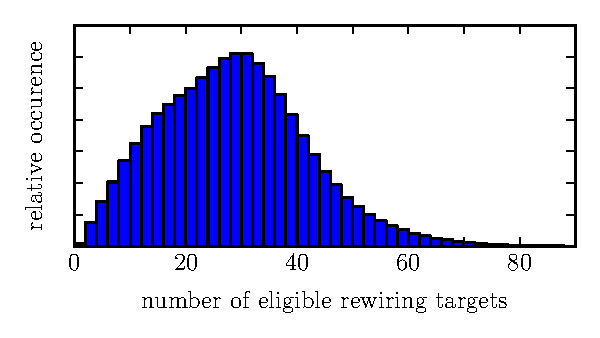
\includegraphics[width=0.8\textwidth]{%
    plots/4afc2727.pdf}
  \caption{(\smtcite{4afc2727})}
  \label{suppfig:rew_stats}
\end{figure}


\subsection*{\autoref{ch:structural_aspects}}

\begin{figure}[H]
  \centering
  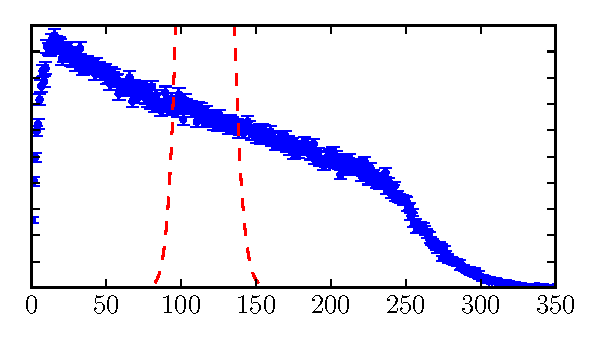
\includegraphics[width=0.7\textwidth]{%
    plots/c7ee86d7.pdf}
  \caption{(\smtcite{c7ee86d7})}
  \label{suppfig:out_degree}
\end{figure}


% \begin{figure}[H]
%   \centering
%   \includegraphics{



%%% Local Variables: 
%%% mode: latex
%%% TeX-master: "../dplths_document"
%%% End: 